\documentclass{ltjsarticle} %lualatex cs_jikken.texで作成 
\usepackage{mdframed}
\usepackage{graphicx}
\usepackage{float}
\usepackage{array}
\usepackage{tikz}
\usepackage{circuitikz}
\usetikzlibrary{automata, positioning, arrows}
\begin{document}

\thispagestyle{empty}
\begin{flushright}
{\large 実施日 2024年11月17日{\hspace{5cm}}} 
\end{flushright}

\vspace*{\fill}
\centering
{\Huge\bf コンピュータ科学実験b}
\vspace*{1cm}

{\huge\bf ソフトウェア実験 第1,2週 調査課題}
\vspace*{\fill}

\vspace*{\fill}

\vspace*{\fill}

\begin{flushright}
{\large 学生番号: 102210017} \\ % 5cmの空白を作り、アンダーラインを引く
{\large 氏名: 安藤 駿} \\

{\large 共同実験者:} \\
\end{flushright}

\clearpage

\addtocounter{page}{-1}
\raggedright
\setlength{\parindent}{1em}


\section{調査課題1 TCP, IPパケットのヘッダ情報}

\subsection{TCPパケットのヘッダ情報}

TCPヘッダの構造は図\ref{fig:TCP}に示すようになっている. 

送信元ポート番号は, 16ビットのフィールドで、0~65535の範囲の値が使用され, 
パケットを送信したアプリケーションを識別するために使用される. 
宛先ポート番号も16ビットのフィールドで, パケットが送信されるアプリケーションやサービスを識別するために使用する. 

シーケンス番号は, 32ビットのフィールドで, TCPセグメントのデータ部が
元データの何バイト目の位置のものかを表すために使用される. 

確認応答番号は, 2ビットのフィールドで、受信側が「次に受信することを想定しているシーケンス番号」を送信側に伝えるために使用される. 

データオフセットは, TCPヘッダのサイズは可変長のため, 受信側にヘッダとデータの境目を正しく伝えるために, 
データフィールドの開始位置を表す、4ビットのフィールドである. 

予約は, 6ビットのフィールドで, 将来のために予約されている. 現在は使用していないため「0」がセットされる. 

制御ビットには, 1ビットのフィールドが6つある. 
URG(Urgent Pointer)は, 1の場合は緊急ポインタフィールドが有効であることを示す. 0の場合は, 緊急ポインタフィールドの値も0になる. 
ACK(Acknowledgement Number)は, 1の場合は確認応答番号フィールドが有効であることを示す. 
つまり, 1の場合は確認応答番号フィールドに0以外の値がセットされている. 
0の場合は, 確認応答番号フィールドの値も0になる. コネクション確立時の最初のSYNパケット以外は, 必ず1でなければならない. 
PSH(Push)は, データを即座にアプリケーションに転送するよう指示するために使用される. 
送信側TCPは, プッシュ機能が指示されるまでデータを送信バッファにためて, 自分の都合が良いときに送信できる. 
RST(Reset)は, コネクションのリセットである. 通常は0がセットされているが, コネクションを一方的に強制終了させるときなどに1をセットして送信する. 
SYN(Synchronize)は, コネクション確立時に使われる. このビットが1の場合, コネクションの確立を要求するとともに, 
シーケンス番号に格納されている数字でシーケンス番号を初期化する. 
FIN(Fin Flag)は, 1の場合以後送信するデータがないことを示す. 通信が終了し, コネクションを切断したい場合に使用する. 

ウインドウは, 16ビットのフィールドで, 受信バッファの空きサイズを受信側が送信側に通知するために使用される. 
送信側では通知された値に従って, 送信パケット数を調整する. 

チェックサムは, 16ビットのフィールドでエラーチェックのためのフィールドである. 

緊急ポインタは, 16ビットのフィールドで, データ部に緊急データが含まれているときに緊急データの位置を受信側に伝えるために使用される. 

オプションは, 必要に応じてオプションを追加できる任意のフィールドである. 

パディングは, TCPヘッダは32ビットの倍数と決められているため, 必要に応じてTCPヘッダのサイズを調整するために使用される. 

(pcap, 2018)

\begin{figure}[H] % 画像を挿入する環境を開始
  \centering
  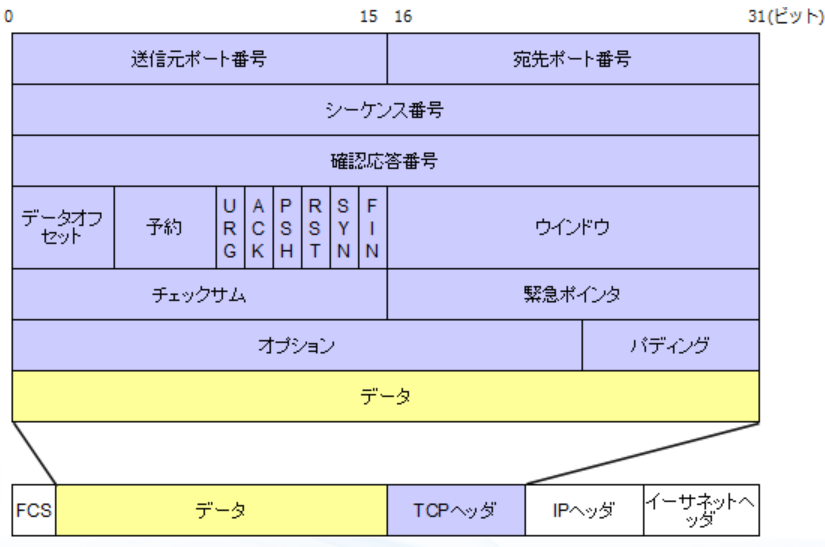
\includegraphics[width=1.0\textwidth]{TCP.png} % 画像を挿入、幅をページ幅に合わせる
  \caption{TCPヘッダの構造} % キャプションを追加
  \label{fig:TCP} % ラベルを追加
\end{figure}

\subsection{IPパケットのヘッダ情報}
IPヘッダの構造は図\ref{fig:IP}に示すようになっている. 

バージョンは, IPのバージョンである. IPv4の場合は「4」がセットされる. 

IPヘッダ長は, 4ビットのフィールドで, IPヘッダのサイズを4で割った値がセットされる. 

サービスタイプ(Type Of Service)は, TOSフィールドとも呼ばれ, QoSを行う場合に利用される. 

IPデータグラム長は, IPデータグラム(IPヘッダ + データ)のサイズをバイト単位で表す. 
IP自体は最大65,535バイトまで扱うことができるが, 実際のIPデータグラムのサイズはデータリンク層のプロトコルが扱えるMTUに依存する. 

ID(Identification), フラグ, フラグメントオフセットは, データリンク層のMTUを超えるような大きいパケットが生成された場合, 
IPはデータリンク層のMTUに合わせてパケットを分割する. 
分割されたパケットは受信側ホストで再構築される. 受信側でパケットが正しく再構築できるように必要な情報を提供するのが, ID, 
フラグ, フラグメントオフセットとなる. 

生存時間(Time To Live:TTL)は, TTLと呼ばれ, 8ビットのフィールドであり, パケットがネットワークに存在できる時間を秒数で表す. 
TTLの値は, 送信元ホストによって初期値が設定され, ルータがパケットを中継するたびに中継処理にかかった秒数(1秒未満の場合は1)ずつ減らされる. 

プロトコルは, 8ビットのフィールドであり, 上位層のプロトコルを番号で表す. 

ヘッダチェックサムは, 16ビットのフィールドで, 受信側でエラーチェックを行うための値がセットされる. 

送信元アドレス(Sorce Address), 宛先アドレス(Destination Address)は, それぞれ32ビットのフィールドで, 
送信元のIPアドレスと宛先IPアドレスがセットされる. 

オプションは, 可変長のフィールドで, テストやデバッグなどを行うときに使用される. 

パディングは, オプションフィールドが32ビットの整数倍にならない場合に、IPヘッダサイズの調整のために0が挿入される使用される. 

(pcap, 2018)

\begin{figure}[H] % 画像を挿入する環境を開始
  \centering
  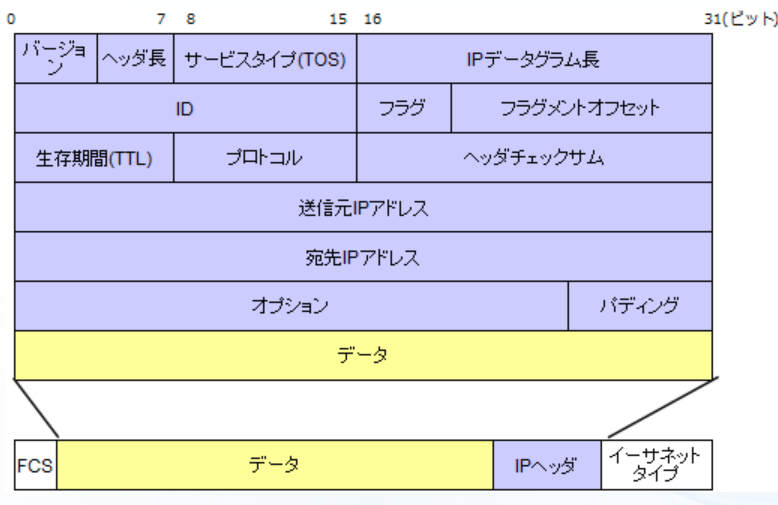
\includegraphics[width=1.0\textwidth]{IP.png} % 画像を挿入、幅をページ幅に合わせる
  \caption{IPヘッダの構造} % キャプションを追加
  \label{fig:IP} % ラベルを追加
\end{figure}



\section{調査課題2 TCP/IP通信におけるブロードキャスト}

\subsection{ブロードキャストの役割}
ブロードキャストとは, ネットワークに接続されている全ての機器に対して, 同じ情報を一度に送信する通信方式のことである. 

\vspace{0.5cm}

ブロードキャストは, ネットワークに接続されたデバイス(コンピュータ、プリンタ、ルータなど)を検出するために利用される. 
例えば,  DHCPクライアントがIPアドレスを取得する際, ネットワーク内のDHCPサーバを見つけるためにブロードキャストを使用する. 

\vspace{0.5cm}

また, 新しいデバイスがネットワークに接続した際, IPアドレスを取得するためにDHCPDISCOVERメッセージをブロードキャストする. 
その結果, DHCPサーバが応答し、デバイスに適切なIPアドレスが提供される. 

(e-words, 2023)

\subsection{ブロードキャストの特徴}
ブロードキャストの特徴は, 一度のデータ送信でネットワークに接続された多数の機器に同時に情報を届けることができることである. 

\vspace{0.5cm}

この特徴は、いくつかの場面でメリットをもたらす. 

まず, 送信元が受信先の機器のアドレスを個別に知らなくても, 情報を届けられることである. 
これは, ネットワークに接続されている機器の数が多い場合や, 接続状況が流動的な場合に特に有効である. 
例えば, 大規模な社内ネットワークや, 不特定多数の機器が接続する公共Wi-Fiなどでも, それぞれの機器のアドレスを把握していなくても, 
ブロードキャストを使えば情報を確実に届けることができる. 

\vspace{0.5cm}

また, 一度の送信ですべての機器に情報を届けられるため, 送信側の負担が軽減されるというというメリットもある. 
個別にデータを送信する場合と比べて、ネットワークの負荷を大幅に減らすことができる. 
これは, ネットワークの帯域幅が限られている場合や, リアルタイム性が求められるシステムにおいて大きな利点になる. 

\vspace{0.5cm}

しかし, デメリットもある. 
ブロードキャストは, ネットワークに接続されているすべての機器に対して, データを送信してしまう.  
これは, 必要なデータを受け取る機器にとっては効率的であるが, 関係のない機器にとっても同様の処理が発生することになるので, 
ットワーク全体の情報量が過剰になり, 処理速度の低下を招く可能性がある. 

\vspace{0.5cm}

また, 攻撃者がブロードキャストを利用して, ネットワーク内のすべてのデバイスに不正なパケットを送信する可能性があり, 
セキュリティが脆弱になることなどの問題が生じることもある. 

(netanzen, 2024)


\section{調査課題3}
PC1 (192.168.200.2) から PC2 (10.10.1.20) への SSH 接続において、TCP パケットが目的地に到達するまでの過程を説明する. 

\subsection{PC1からの送信情報}
TCP/IP プロトコルを使用して、PC1 は SSH(ポート番号 22)の通信を開始する. 

パケットに含まれている情報は, 送信元 IP アドレス(192.168.200.2), 送信元ポート(動的に割り当てられる), 
宛先 IP アドレス(10.10.1.20), 宛先ポート(22)などである. 

\subsection{ARPプロトコルによるMACアドレス解決}
PC1 が最初に ARP プロトコルを使用して、ルータ(デフォルトゲートウェイ)の MAC アドレスを取得する. 
これにより、Ethernet フレームに適切な宛先 MAC アドレスが設定される. 

\subsection{LANルータ(192.168.200.1)での処理}
PC1から受信したパケットをチェックし、宛先IP(10.10.1.20)が異なるネットワークに属していると判断する. 
ルーティングテーブルを参照し、パケットをFW構築実験用ルータ(192.168.100.1)に転送する. 

\subsection{FW構築実験用ルータ(192.168.100.1)の処理}
192.168.100.1 のファイアウォール(icesc01)が受信パケットを検査する. 
SSH通信(TCP 22番ポート)が許可されている場合のみ、転送を実行する. 

パケットを教育用計算機システムネットワーク(10.10.0.0/16)に送信する. 

\subsection{教育用計算機システムネットワークへの到達}
192.168.100.1から送信されたパケットが、教育用計算機システムネットワーク内のルータ(icesc20, IP: 10.10.1.255)に到達する. 
ルータ(icesc20)はパケットを最終的な宛先PC2(10.10.1.20)に転送する. 

\subsection{PC2での受信}
PC2(10.10.1.20)がSSHパケットを受信し、TCP接続の確立を試みる. 
成功すると、SSH 接続が開始される. 

\subsection{ルーティング情報}
各ルータ(各班用ルータ, FW構築実験用ルータ)はルーティングテーブルを保持しており, 
宛先IPアドレスに基づいて次に転送すべきネットワークインターフェースを判断する. 

各ネットワーク間をつなぎ、パケットを目的地まで確実に届ける. 

\subsection{ブロードキャストの役割}
ネットワーク内で新しいデバイスのIPアドレスを解決する際, ARP(Address Resolution Protocol)でブロードキャストが利用される. 
例えば, PC1が「各班用ルータのMACアドレス」を取得するために ARP リクエストを送信し, その応答を得る形で通信が開始される. 



\section{調査課題4 DNS の詳細}

\subsection{DNS(Domain Name System)とは}
DNS(Domain Name System)とは, インターネットなどのIPネットワーク上でドメイン名とIPアドレスの対応関係を管理するシステムである. 
利用者が単なる番号列であるIPアドレスではなく, 日常使っている言語の文字を組み合わせた認識しやすいドメイン名で, 
ネットワーク上の資源にアクセスすることができるようになる. 

\vspace{0.5cm}

例えば, ある企業が「198.51.100.1」というIPアドレスの割り当てを受けてWebサーバと電子メールサーバを運用する場合, 
WebサイトのURLは「https://198.51.100.1/」のようになり, 代表メールアドレスは「info@198.51.100.1」のような表記になる. 
これは人間にとっては覚えたり伝達したり入力したりしにくい. 

\vspace{0.5cm}

また, 接続事業者を切り替えるなどしてIPアドレスが替わるとこれらのアドレスもすべて変更となり, 
記録物を書き直したり関係者に改めて通知・告知しなおさなければならなくなってしまう. 

\vspace{0.5cm}

そこで, 「example.co.jp」というドメイン名を取得し, ホスト名として「www.example.co.jp」を「198.51.100.1」に, 
「~@example.co.jp」のメールアドレスを管理するメールサーバのアドレスを「198.51.100.1」に対応付けておけば, 
これらの問題を解決できる. 

\subsection{DNSの基本的な仕組み}
DNSクライアント(リゾルバ)が, ユーザーがウェブサイトにアクセスする際に, 最初にDNSリクエストを送信する. 
そして, DNSサーバーが, このリクエストを受け取り、適切なIPアドレスを返すことで, ドメイン名とIPアドレスが対応付けされる. 

(e-words, 2023)


\subsection{DNSのセキュリティ強化の動向}
DNSのセキュリティ強化のための技術として, DNSSECがある. 
DNSSEC(Domain Name System Security Extensions)は, DNSデータの完全性と認証を提供するための技術である. 

\vspace{0.5cm}

この技術により, DNSの応答が改ざんされていないことを確認できる. 
具体的には, DNSリソースレコード(RR)の応答にデジタル署名を追加し, リゾルバが署名を検証することで, 
偽のDNSレコード(例: フィッシング攻撃による偽サイトのリダイレクト)を防止することができる. 

DNSSECでは、DNSレコードにデジタル署名を追加する. 
これにより、DNSデータが正当であるかどうかを確認するための署名が生成される. 

公開鍵と秘密鍵のペアを使用して, DNSデータを署名する. 
ドメインの権威DNSサーバーは, 秘密鍵を使ってDNSレコードを署名し, その署名を含む応答をリゾルバに返す. 
DNSレコードに署名するために使用され, 秘密鍵が漏洩しないように厳重に管理される. 
DNSリゾルバがDNSレコードの署名を検証するために使用され, 
公開鍵はDNSレコードに含まれているか, 上位の権威サーバーから取得される. 

(nesuke, 2023)


\section{調査課題5 暗号化を行うプロトコル}

\subsection{SMTP}
SMTP(Simple Mail Transfer Protocol)は, メールを送信するために使われるプロトコルのことである. 

\vspace{0.5cm}

SMTP は1980年代から使われている古いプロトコルで, 最初の仕様はIETFによって1982年にRFC 821として規格化された. 
幾度かの改訂を経て2008年に最新版のRFC 5321が発行されている. 
1994年に追加された拡張機能やコマンド群は「ESMTP」(SMTP Service Extensions)と呼ばれることもある. 

\vspace{0.5cm}

暗号化の仕組みには, STARTTLSなどがあり, これはSMTP通信の途中でTLS暗号化を開始する方式である. 
暗号化がサポートされていない場合は通常の通信にフォールバックする. 

また, SMTPS(SMTP over SSL/TLS)は, 通信の開始時からTLSを使用して暗号化する方式である. 

(baremail, 2021)

\subsection{IMAP}
IMAP(Internet Message Access Protocol)は、インターネットなどのIPネットワークで標準的に用いられる, 
電子メールを受信するためのプロトコルである. 
利用者が自分宛ての電子メールを保管しているメール受信サーバにアクセスし, 新着を確認したり一覧から必要なものを選んで手元に受信する手順を定めている. 

\vspace{0.5cm}

最も初期のバージョンはIETFが1988年にRFC 1064として策定したIMAP2だが, 正式名称は現在と異なり Interactive Mail Access Protocol だった. 
1994年にIMAP4がRFC 1730として策定され, このとき現在の名称に改められた. 
IMAP4は最も普及したバージョンであり, 単にIMAPといった場合はIMAP4を指すことが多い. 
IMAP4には様々な拡張仕様が追加され, 2003年にはRFC 3501として改訂されている. 

\vspace{0.5cm}

暗号化の仕組みには, IMAP over SSL/TLSがあり, これは, IMAPでTLS暗号化を使用する方式である. 

また, POP3 over SSL/TLSは, POP3でTLS暗号化を使用する方式である. 

(e-words, 2021)


\subsection{FTP}
FTP(File Transfer Protocol)は, ネットワーク上でファイルを送受信する際に使用する通信プロトコルである. 

FTPサーバーに作成したファイルをアップロードすることで, 新規のWebページを追加できる. 
また, 既存ファイルの一部を書き換えたものをアップロードし, サーバー上の既存ファイルに上書きすれば, 公開済みのページの内容を更新することも可能である. 

\vspace{0.5cm}

暗号化の仕組みには, FTPS(FTP Secure)があり, これはSSL/TLSを使用して通信を暗号化したFTPの拡張版である. 

また, SFTP(SSH File Transfer Protocol)は, SSHプロトコルを使用してセキュアな通信を行う別の方式である. 

(kagoya, 2024)



\begin{thebibliography}{99} % 最大ラベル幅を99に設定
    
  \bibitem{lamport1994latex}
  pcap: 
  \emph{TCPプロトコル}. \\
  \verb|https://pcap.it-mem.info/プロトコル/tcpプロトコル/|  2018. 

  \bibitem{lamport1994latex}
  pcap: 
  \emph{IPプロトコル}. \\
  \verb|https://pcap.it-mem.info/プロトコル/ipプロトコル/|  2018. 

  \bibitem{lamport1994latex}
  e-words: 
  \emph{ブロードキャスト}. \\
  \verb|https://e-words.jp/w/ブロードキャスト.html|  2023. 

  \bibitem{lamport1994latex}
  netanzen: 
  \emph{ブロードキャストとは?誰でもわかるネットワーク通信の基本}. \\
  \verb|https://netanzen.jp/network/understanding-broadcast-a-basic-network-communication-method/|  2024. 

  \bibitem{lamport1994latex}
  e-words: 
  \emph{DNS 【Domain Name System】 ドメインネームシステム}. \\
  \verb|https://e-words.jp/w/DNS.html|  2023. 

  \bibitem{lamport1994latex}
  nesuke: 
  \emph{初心者にも分かりそうなDNSSECの仕組みと機能}. \\
  \verb|https://milestone-of-se.nesuke.com/l7protocol/dns/dnssec-summary/|  2023. 

  \bibitem{lamport1994latex}
  baremail: 
  \emph{SMTPとは? メール送受信の基礎知識と、SMTPサーバーの機能と課題}. \\
  \verb|https://baremail.jp/blog/2021/04/05/1217/|  2021. 

  \bibitem{lamport1994latex}
  e-words: 
  \emph{IMAP 【Internet Message Access Protocol】 IMAP4}. \\
  \verb|https://e-words.jp/w/IMAP.html|  2020. 

  \bibitem{lamport1994latex}
  kagoya: 
  \emph{FTPとは?通信の仕組みやソフトについてわかりやすく解説}. \\
  \verb|https://www.kagoya.jp/howto/it-glossary/web/ftp/|  2024. 

\end{thebibliography}


\end{document}